\noindent

\includegraphics[height=1.25cm]{images/pictograms/replication}

\includegraphics[height=1.25cm]{images/pictograms/benchmark}

\includegraphics[height=1.25cm]{images/pictograms/under_construction}

\includegraphics[height=1.25cm]{images/pictograms/msc}

\includegraphics[height=1.25cm]{images/pictograms/FDM}
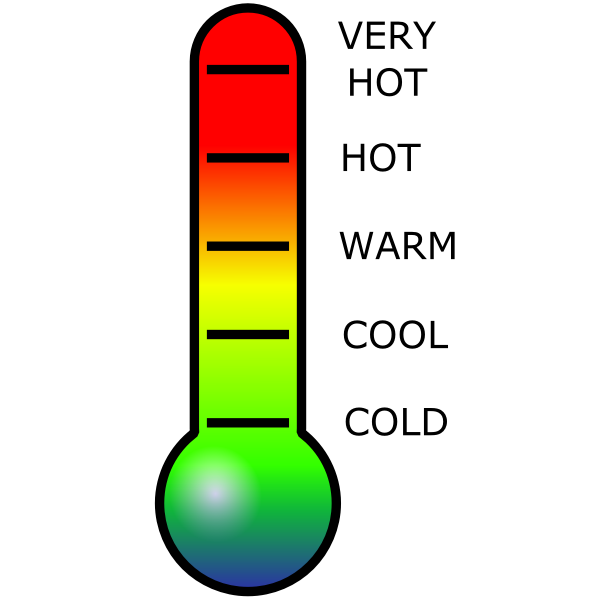
\includegraphics[height=1.25cm]{images/pictograms/temperature}

\includegraphics[height=1.25cm]{images/pictograms/paraview}

%%%%%%%%%%%%%%%%%%%%%%%%%%%%%%%%%%%%%%%%%%%%%%%%%%%%%%%%%%%%%%%%%%%%%%%%%%%%%%%%%%%%%%%%%%%%%%%%%%%

\begin{flushright} {\tiny {\color{gray} python\_codes/fieldstone\_152/text.tex}} \end{flushright}

%\lstinputlisting[language=bash,basicstyle=\small]{python_codes/template_keywords.key}

\par\noindent\rule{\textwidth}{0.4pt}

\begin{center}
\inpython
{\small Code: \url{https://github.com/cedrict/fieldstone/tree/master/python_codes/fieldstone_152}}
\end{center}

\par\noindent\rule{\textwidth}{0.4pt}

{\sl This stone was developed in collaboration with C. Leblanc and F. Gueydan}. 
\index{contributors}{F. Gueydan}
\index{contributors}{C. Leblanc}

\par\noindent\rule{\textwidth}{0.4pt}

%%%%%%%%%%%%%%%%%%%%%%%%%%%%%%%%%%%%%%%%%%%%%%%%%%%%%%%%%%%%%%%%%%%%%%%%%%%%%%%%%%%%%%%%%%%%%%%%%%%

The setup is based on \textcite{vack08} (2008). This benchmark is carried out in \stone~68 and 149.
The code was developed during the MSc thesis of C. Leblanc. 

DESCRIBE

this is case 1a. 


\begin{center}
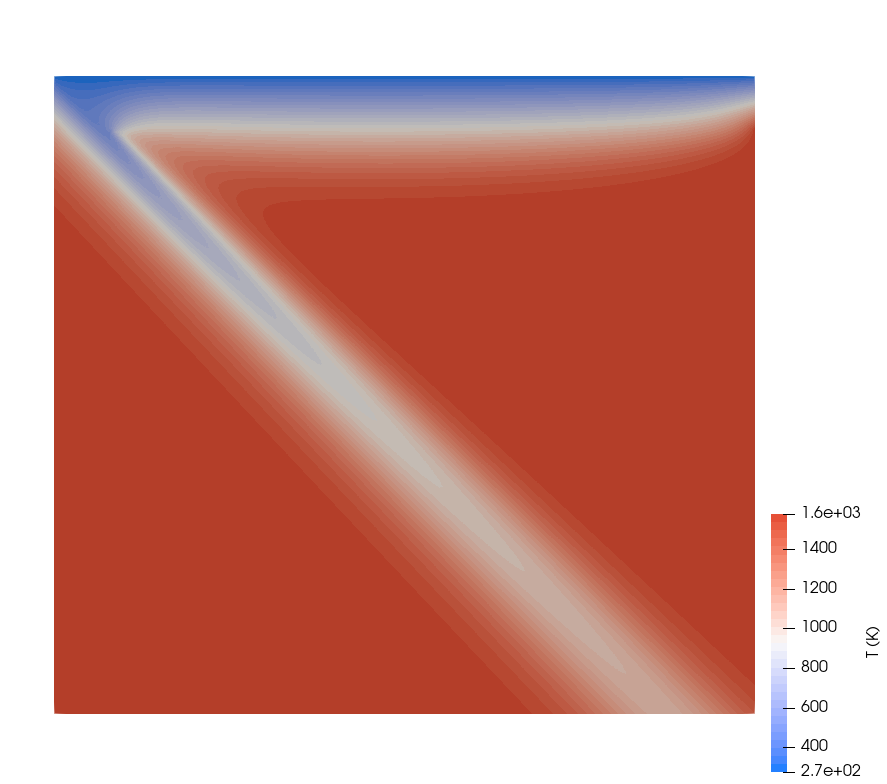
\includegraphics[width=8cm]{python_codes/fieldstone_152/results/T}
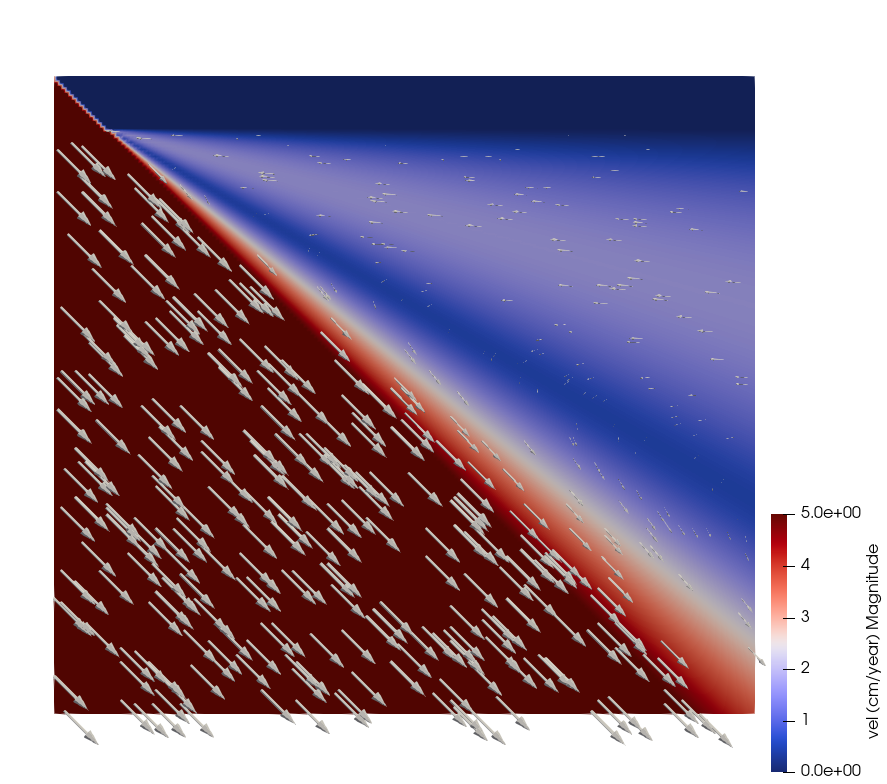
\includegraphics[width=8cm]{python_codes/fieldstone_152/results/vel}
\end{center}









